\section{}
% In order to avoid boundary layer interference, engineers design a “boundary layer 
% scoop” to skim off the boundary layer in a large wind tunnel (see Figure 1). The 
% scoop is constructed of thin sheet metal. The air is at 20°C and flows at 𝑉 =
% 45.0 m/s. How high (dimension ℎ) should the scoop be at downstream distance 
% 𝑥 = 1.45 m?

\textit{In order to avoid boundary layer interference, engineers design a “boundary layer scoop” to skim off the boundary layer in a large wind tunnel (see Figure 1). The scoop is constructed of thin sheet metal. The air is at 20°C and flows at $V = 45.0 m/s$. How high (dimension $h$) should the scoop be at downstream distance $x = 1.45 m$?}

\begin{figure}[H]
    \centering
    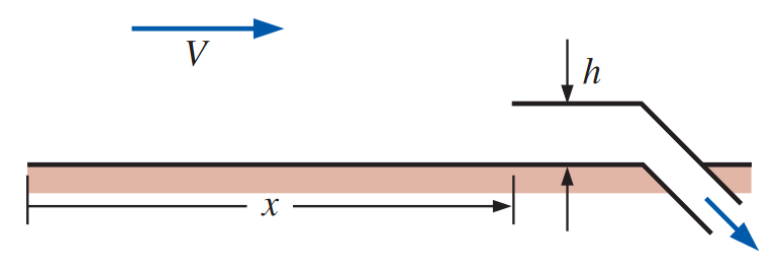
\includegraphics[width=0.5\textwidth]{Questions/Figures/Q2 Problem Diagram.png}
    \caption{Boundary Layer Scoop}
\end{figure}

First, calculate the Reynolds number at $x = 1.45 m$. The kinematic viscosity of air at $20^\circ C$ is $\nu = 1.516 \times 10^{-5} m^2/s$ \cite{cengel_fluid_2018}.
\begin{equation*}
    \text{Re}_x = \frac{Vx}{\nu} = \frac{45.0 \times 1.45}{1.516 \times 10^{-5}} = 4.30 \times 10^6
\end{equation*}
This is past the $\text{Re}_{\text{engineer}} = 5 \times 10^5$ threshold, so this is turbulent. Using the turbulent boundary layer thickness equation,
\begin{align*}
    \frac{\delta}{x} &= \frac{0.16}{\text{Re}_x^{1/7}} \\
    &= \frac{0.16}{(4.30 \times 10^6)^{1/7}} \\
    &= 0.0181 \times 10^{-3} 
\end{align*}
Then,
\begin{align*}
    \delta &= 0.0181 \times 10^{-3} \times 1.45 \\
    &= 2.62 \times 10^{-5} \\
    &= \boxed{26.2 \text{ mm}}
\end{align*}
So the scoop should be at least 26.2 mm high at $x = 1.45$m.